\chapter{任务目标}

本次课程设计的任务是基于谣言检测数据集,构建一个检测模型。该模型可以对数据集中的推文进行谣言检测与识别。要求如下:
\begin{itemize}
    \item 数据集:使用给定的谣言检测数据集,数据集包含推文文本和标签(谣言或非谣言)。
    \item 训练模型:使用逻辑回归或GRU等深度学习模型进行谣言检测,实现二分类任务,
    用0代表非谣言、1代表谣言
    \item 泛化能力:模型应具有较好的泛化能力,能够适应不同类型的谣言检测任务。
    \item 评估指标:分类准确率、运行时间等
    \item 结果可视化:对模型训练结果进行可视化展示。
\end{itemize}

\vspace{1em}

我们需要在接口类文件classify.py中实现接口类RumourDetectClass,该类对外提供一个接口函数classify,该函数接收一条字符串作为输入,输出一个int值作为对应的预测类别。该类共包含以下方法:
\begin{itemize}
    \item \verb|__init__(self, model_path, vocab_path, EMBEDDING_DIM = 128, |\\
    \verb|HIDDEN_DIM = 256, DEVICE = NONE)|: 初始化,加载指定词表和模型参数
    \item \verb|construct_detector(self)|: 无参数快速构建谣言检测器,加载默认模型和词表
    \item \verb|classify(self, text)|: 对输入文本进行预测,返回预测结果
\end{itemize}

\chapter{具体内容}

\section{实施方案}

在经过小组成员的讨论后,我们决定采用改进型双向长短时记忆网络(AdvancedBiLSTM3)模型开展谣言检测任务。该模型在传统BiLSTM基础上,结合了注意力机制、Dropout正则化和LayerNorm等技术,能够更好地捕捉文本的上下文依赖关系,并有效缓解过拟合问题。具体改进如下:

\begin{itemize}
    \item \textbf{嵌入层与Dropout:} 在词嵌入层后增加Dropout,有效防止特征过拟合。
    \item \textbf{简化LSTM结构:} 采用双向LSTM,隐藏层维度减半后拼接,保持总输出维度不变,层数限制为2层,提升模型效率。
    \item \textbf{注意力机制:} 引入带有中间层和Dropout的注意力机制,突出关键信息,提升模型对长文本的理解能力,并对padding部分进行mask处理,避免无效信息干扰。
    \item \textbf{分类器正则化:} 分类器部分加入多层Dropout和LayerNorm,增强模型泛化能力。
\end{itemize}

与传统的BiGRU或逻辑回归模型相比,AdvancedBiLSTM3模型具备更强的特征表达能力和鲁棒性,能够自动学习文本中的复杂语义关系,适应不同领域的谣言检测任务。通过注意力机制,模型能够聚焦于文本中的关键信息片段,提升对谣言特征的捕捉能力。实验结果表明,该模型在准确率和泛化能力方面均优于传统方法。

\section{核心代码分析}

\subsection{训练模型train\_lstm.py}
\begin{codeblock}[language=Python]
import re
from train_gru import *

class RumourDetectClass:
    def __init__(self):
        # 加载词表和模型参数
        self.vocab = build_vocab(pd.read_csv('../dataset/split/train.csv')['text'])
        self.model = BiGRU(len(self.vocab), EMBEDDING_DIM, HIDDEN_DIM).to(DEVICE)
        self.model.load_state_dict(torch.load('../Output/bigru.pt', map_location=DEVICE))
        self.model.eval()

    def preprocess(self, text):
        # 文本预处理(与训练时一致)
        text = re.sub(r'[^\w\s]', '', text.lower())
        return text
    
    def classify(self, text: str) -> int:
        # 预测流程
        text = self.preprocess(text)
        ids = encode(text, self.vocab)
        x = torch.tensor([ids], dtype=torch.long).to(DEVICE)
        with torch.no_grad():
            logits = self.model(x)
            pred = (torch.sigmoid(logits) > 0.5).float().item()
        return int(pred)
\end{codeblock}


\subsection{接口类classify.py}
\begin{codeblock}[language=Python]
import torch
import re
from train_gru import *

class RumourDetectClass:
    def __init__(self, model_path):
        # 加载词表和模型参数
        self.vocab = joblib.load(vocab_path)
        self.model = BiGRU(len(self.vocab), EMBEDDING_DIM, HIDDEN_DIM).to(DEVICE)
        self.model.load_state_dict(torch.load(model_path, map_location=DEVICE))
        self.model.eval()

    def preprocess(self, text):
        # 文本预处理(与训练时一致)
        text = tokenize(text)
        ids = encode(text, self.vocab)
        return ids
    
    def classify(self, text: str) -> int:
        # 预测流程
        ids = self.preprocess(text)
        x = torch.tensor([ids], dtype=torch.long).to(DEVICE)
        with torch.no_grad():
            logits = self.model(x)
            pred = (torch.sigmoid(logits) > 0.5).float().item()
        return int(pred)
\end{codeblock}

\section{测试结果分析}


\begin{figure}[ht]
  \centering
  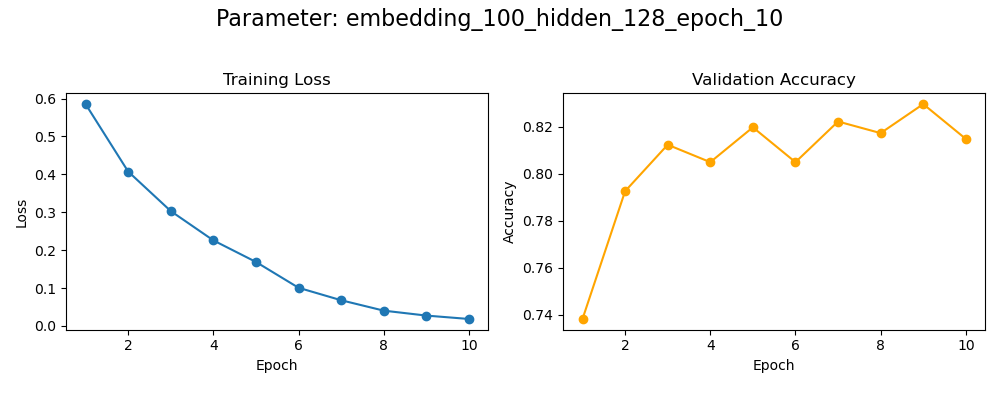
\includegraphics[width=0.8\textwidth]{../Output/Graph/embedding_100_hidden_128_epoch_10.png}
  \caption{embedding\_100\_hidden\_128\_epoch\_10}
\end{figure}




\chapter{工作总结}

\section{收获与心得}

通过本次课程设计,我深入学习了深度学习模型在自然语言处理中的应用,特别是双向门控循环单元(BiGRU)模型在文本分类任务中的优势。通过对比不同模型的性能,我认识到模型的选择对任务结果的影响。此外,我还掌握了数据预处理、模型训练和评估等一系列技能,为今后的研究奠定了基础。

\section{遇到问题及解决思路}

在项目实施过程中,我遇到了一些问题,例如数据集不平衡导致模型偏向于某一类标签。为了解决这个问题,我尝试了数据增强和调整损失函数等方法,最终通过对训练数据进行重采样,取得了较好的效果。

此外,我还遇到了一些模型训练过程中的技术问题,例如梯度消失和过拟合等。为了解决这些问题,我尝试了不同的优化算法和正则化方法,最终通过调整学习率和使用Dropout等技术,成功提高了模型的性能。

\chapter{课程建议}

本次课程设计通过实践操作,让我们对深度学习与自然语言处理的结合应用有了具象认知,但在课程学习及实践过程中,也发现一些可以优化改进的方向,此处提出几点建议,希望能为后续课程设计提供参考:

当前课程较多聚焦于基础概念的介绍讲解,但对具体算法的原理推导与代码实现讲解较少,部分概念比较晦涩难懂但缺乏深入剖析,导致学生在理解上存在困难。希望老师能结合代码实例进行拆解演示,如结合 PyTorch 等库的具体实现,深入讲解 GRU、LSTM 等模型的工作原理与数学推导,帮助学生更好地理解模型背后的逻辑。

此外,本课程前期未铺垫相关实践案例,而课程设计在学期末才公布,与其他课程结课任务、考试复习等时间冲突,导致学生难以分配足够精力深入探索,也是我认为可以改进的地方。在本次课程设计中,我们小组成员普遍感受到时间紧迫,从理解任务、数据预处理到模型调优全程压缩在短时间内,尤其是在数据预处理、模型训练与调优等环节,难以进行充分的实验与探索。建议将课程设计主题提前半学期公布,分阶段设置任务节点(如第 8 周完成数据预处理、第 12 周提交模型初版等),并配套阶段性指导,帮助学生合理规划时间,确保实践质量。

而在完成项目的过程中,我们也意识到仅凭课堂上学到的知识,难以独立完成整个项目,特别是对 PyTorch 、Sklearn 等库的使用不够熟悉,导致在实现过程中遇到很多问题。建议老师能在前期的课程中结合具体案例,帮助学生更好地掌握这些工具的使用方法。